\section{Reachi Experiments}
\todo[inline]{introduce the data. WIP}
To verify that our model for computing path loss gives proper results, we have received data from conducted
experiments from the Reachi project. In total we have received data from four experiments. Three experiments
was conducted with 33 devices, while the fourth with 330.
% OMG SO BAAAAAD

\todo[inline]{talk about the problems with the data. WIP}
When we detected odd behaviour, we started to investigate the logs. Specifically the logs from experiments
conducted in Marikina and Rude Skov. The reason for these two, is that the Rude Skov log was not conducted in
the middle of a city while the Marikina was, as such the Marikina log should contain more varying signal
strength measurements because there is more dense obstructions that can influence the signal. We used the
distance dependent fading function from \cite{paper:linkmodel}, that computes path loss based on the distance
of a link, where we compared the measurements with transmission power - path loss computed from the distance
fading function.

On plot \ref{plot:reachi-experiments:average-distance} the measurements and distance fading function RSSI
values can be seen. The measurements have been divided into distance buckets, where the average for each
bucket has been computed and plotted.

\begin{figure}[H]
    \centering
    \begin{tikzpicture}%\label{plot:reachi-experiments:average-distance}
        \begin{axis}[
                height=12cm, width=0.95\textwidth,
                ylabel={RSSI},
                xlabel={Distance in meters},
                axis lines*=left,
                xmin=0, xmax=750,
                enlargelimits=false,
                ymin=-120, ymax=-20,
                xtick={0, 50, 100, 150, 200, 250, 300, 350, 400, 450, 500, 550, 600, 650, 700, 750},
                ymajorgrids=true,
                xmajorgrids=true,
                grid style=dashed,
                restrict y to domain=-120:-20,
                samples=600
            ]

            \addplot[very thick, solid, cyan, mark=*] coordinates {(20, -28.32345013477089) (40, -44.85830258302583) (60, -52.77323717948718) (80, -60.21201657458563) (100, -66.47435897435898) (120, -69.68905472636816) (140, -71.5976496922216) (160, -73.7866473149492) (180, -75.53428571428572) (200, -76.89289392378991) (220, -77.88135593220339) (240, -77.8035019455253) (260, -77.36784140969164) (280, -77.14030612244898) (300, -77.75299760191847) (320, -79.71686746987952) (340, -79.15481171548117) (360, -79.90728476821192) (380, -81.30909090909091) (400, -81.79746835443038) (420, -81.52272727272727) (440, -79.2) (460, -79.42105263157895) (480, -79.4375) (500, -79.0) (520, -77.91666666666667) (540, -83.0) (560, -81.27272727272727) (580, -83.57142857142857) (600, -86.0) (620, -83.4) (640, -86.5) (660, -81.42857142857143) (680, -79.0) (700, -82.71428571428571) (740, -77.0)};
            \addlegendentry{Marikina field measurements};


            \addplot[domain=0:740, very thick, solid, red] {26 - ld(x)};
            \addlegendentry{distance path loss function};
        \end{axis}
    \end{tikzpicture}
    \caption{Average RSSI pr. distance}\label{plot:reachi-experiments:average-distance}
\end{figure}


\begin{figure}[H]
    \centering
    \begin{tikzpicture}%\label{plot:reachi-experiments:average-distance}
        \begin{axis}[
                title=score - 350.722,
                height=12cm, width=0.95\textwidth,
                ylabel={RSSI},
                xlabel={Distance in meters},
                axis lines*=left,
                xmin=0, xmax=380,
                enlargelimits=false,
                ymin=-90, ymax=-30,
                ymajorgrids=true,
                xmajorgrids=true,
                grid style=dashed,
                samples=400
            ]

            \addplot[very thick, solid, cyan, mark=*] coordinates {(20, -32.56521739130435) (40, -50.607142857142854) (60, -52.15384615384615) (80, -64.85714285714286) (100, -49.5) (120, -65.76623376623377) (140, -69.38888888888889) (160, -72.05714285714286) (180, -69.3125) (200, -78.83333333333333) (220, -76.84) (240, -75.75) (260, -80.91666666666667) (280, -72.88888888888889) (300, -78.95238095238095) (320, -76.44444444444444) (340, -82.75) (380, -87.0)};
            \addlegendentry{Marikina field measurements};

            \addplot[domain=0:380, very thick, solid, red] {26 - bopl(x)};
            \addlegendentry{\gls{bopl}};


        \end{axis}
    \end{tikzpicture}
    \caption{Field measurements with building percentage above 80\%}
    \label{plot:reachi-experiments:marikina-log-above-80-pct}
\end{figure}




\begin{figure}[H]
    \centering
    \begin{tikzpicture}%\label{plot:reachi-experiments:average-distance}
        \begin{axis}[
                title=score - 501.586,
                height=12cm, width=0.95\textwidth,
                ylabel={RSSI},
                xlabel={Distance in meters},
                axis lines*=left,
                xmin=0, xmax=750,
                enlargelimits=false,
                ymin=-90, ymax=-30,
                xtick={0, 50, 100, 150, 200, 250, 300, 350, 400, 450, 500, 550, 600, 650, 700, 750},
                ymajorgrids=true,
                xmajorgrids=true,
                grid style=dashed,
                samples=700
            ]

            \addplot[very thick, solid, cyan, mark=*] coordinates {(20, -36.01344537815126) (40, -48.361111111111114) (60, -54.93279022403259) (80, -62.40816326530612) (100, -68.14871794871794) (120, -60.85954712362301) (140, -71.69568452380952) (160, -74.36896551724138) (180, -73.93817204301075) (200, -75.09929078014184) (220, -73.38403041825094) (240, -75.43994413407822) (260, -77.69102990033223) (280, -77.31512605042016) (300, -75.7751937984496) (320, -78.60714285714286) (340, -78.38524590163935) (360, -78.52459016393442) (380, -77.34285714285714) (400, -80.96153846153847) (420, -81.03571428571429) (440, -80.41379310344827) (460, -74.18181818181819) (480, -79.9090909090909) (500, -79.75) (520, -77.56521739130434) (540, -81.23076923076923) (560, -78.9) (580, -85.0) (620, -82.5) (640, -82.33333333333333) (660, -82.4) (680, -77.5) (700, -85.4) (740, -77.0)};
            \addlegendentry{Marikina field measurements}


            \addplot[domain=0:740, very thick, solid, red] {26 - cvpl(x)};
            \addlegendentry{\gls{cvpl}};


        \end{axis}
    \end{tikzpicture}
    \caption{Field measurements with building percentage below 5\%}
    \label{plot:reachi-experiments:marikina-log-below-5-pct}
\end{figure}


\section{Line of Sight Model (LoSModel)}
\todo[inline]{ref to section where field experiments problems discussed}
To facilitate the problems mentioned in \ref{sec:}, we have developed our own model for computing path loss.
The model, called \gls{losmodel}, computes path loss based on the distance of the link and the percentage of
the link that contains building. The idea is that large obstructions, like buildings, cause more severe loss
of signal strength compared to pure distance. Our model only consider buildings as an obstruction, and is
therefore to be taking as a proof of concept.\medbreak

To do the computation, we introduce two deterministic functions for computing path loss. \gls{bopl} computes
path loss for 100\% building obstruction. \gls{cvpl} computes path loss for 0\% building obstruction. They are
combined with the following formula:
\begin{eq}
    pl(link, bp) = (cvpl(\theta(link)) * (100 - bp)) + (bopl(\theta(link)) * bp)
\end{eq}





To compute the building percentage, one could utilize 3D models of area and develop a complex model for
determining the building percentage. However such a solution is computationally expensive, and this projects
scope is scalability. Therefore we propose a simpler solution. The idea is to generate an image of an area
from a map and look at the colour of the pixel, then compute the percentage of total pixels of the link and
the amount of pixels that were coloured as a building.


\begin{eq}
    \mathit{cvpl}(l) = (48.5 * (\ln(d(l)) / \ln(77)) + 37.5);
\end{eq}

\begin{eq}
    \mathit{bopl}(l) = (67 * (\ln(d(l)) / \ln(57)) + 11.5);
\end{eq}



\begin{algorithm}[H]
    \DontPrintSemicolon
    \SetKwFunction{FLoSModelCompute}{ComputePathloss}
    \SetKwProg{Fn}{Function}{}{}

    %Link = $(\mathit{id},\ n_1,\ n_2)$\;
    %PixelPos = $(\mathit{x},\ \mathit{y})$\;\;
    
    %$\mathit{building\_colours}\ \leftarrow$ A set of colours that represent a building in the image\;
    $\mathit{map} \leftarrow$ A map of an area\; %should contain link
    \;
    \Fn{\FLoSModelCompute{$l$}}{
        $n_1, n_2 \leftarrow \mathit{nodes}(l)$\;
        $p_1 \leftarrow$ compute pixel position on $\mathit{map}$ for $n_1$\;
        $p_2 \leftarrow$ compute pixel position on $\mathit{map}$ for $n_2$\;
        $\mathit{bearing} \leftarrow$ compute bearing between $p_1$ and $p_2$\;
        $\mathit{pixels} \leftarrow 0$\;
        $\mathit{buildings} \leftarrow 0$\;
        $x \leftarrow p_{2,x}$\;
        $y \leftarrow p_{2,y}$\;
        \;
        \While{$x \geq p_{1,x}$ \KwAnd $y \geq p_{1,y}$}{
            $\mathit{colour} \leftarrow$ get colour of $(x, y)$ on $\mathit{map}$\;
            \If{$\mathit{colour}$ \KwIs building}{
                $\mathit{buildings} \leftarrow \mathit{buildings} + 1$\;
            }
            $x \leftarrow x - 1$\;
            $y \leftarrow y - \mathit{bearing}$\;
            $\mathit{pixels} \leftarrow \mathit{pixels} + 1$\;
        }
        \;
        $\mathit{pct} \leftarrow \mathit{buildings} / \mathit{pixels}$\;
        $\mathit{pl}_l \leftarrow (\mathit{cvpl}(l) \cdot 1 - pct) + (\mathit{bopl}(l) \cdot pct)$\;
    
        \KwRet $\mathit{pl_l}$\;
        
        
        % $\mathit{bearing} \leftarrow$ compute the bearing from the line created from pos1 and pos2\;
        % $\mathit{tp} \leftarrow 0$\;
        % $\mathit{bp} \leftarrow 0$\;\;

        % $\mathit{x},\ \mathit{y}\ \leftarrow \mathit{pos_2}$\;
        % \While{$\mathit{x} >= \mathit{pos_1.x}\ \KwAnd\ \mathit{y} >= \mathit{pos_1.y}$}{
        %     $\mathit{colour} \leftarrow\ map.get\_colour(\mathit{x},\ \mathit{y})$\;
        %     \If{$\mathit{colour} \in \mathit{building\_colours}$}{
        %         $\mathit{bp} \leftarrow \mathit{bp}\ +\ 1$\;
        %     }
        %     $\mathit{x} \leftarrow \mathit{x}\ -\ 1$\;
        %     $\mathit{y} \leftarrow \mathit{y} \-\ (1 \cdot \mathit{bearing})$\;
        %     $\mathit{tp} \leftarrow \mathit{tp}\ +\ 1$\;
        % }
        % $\mathit{pct} \leftarrow (100 \cdot \mathit{bp})\ /\ \mathit{tp}$\;
        % $\mathit{distance} \leftarrow\ d(link)$\;\;
        % $\mathit{pl_{cv}} \leftarrow cvpl(\mathit{distance}) \cdot (100 - pct)$\;
        % $\mathit{pl_{bo}} \leftarrow bopl(\mathit{distance}) \cdot pct$\;\;

        % \KwRet $\mathit{pl_{cv}} + \mathit{pl_{bo}}$\;
    }
    \caption{The ComputePathloss function.}
    \label{algo:}
\end{algorithm}




To develop the \gls{losmodel}, two deterministic functions had to be computed. \gls{cvpl}, a function for computing the path loss for a signal with nothing obstructing the signal. \gls{bopl}, a function for computing the path loss for a signal with obstructions like buildings. To accomplish that, data was collected from the Marikina log. Links created from the measurements with a building percentage of above 80\% and below 5\% was collected.
The Marikina log was chosen, because the field measurements are from within a city thereby giving

In \autoref{plot:reachi-experiments:marikina-log-above-80-pct} and \autoref{plot:reachi-experiments:marikina-log-below-5-pct}.





\begin{figure}[H]
    \centering
    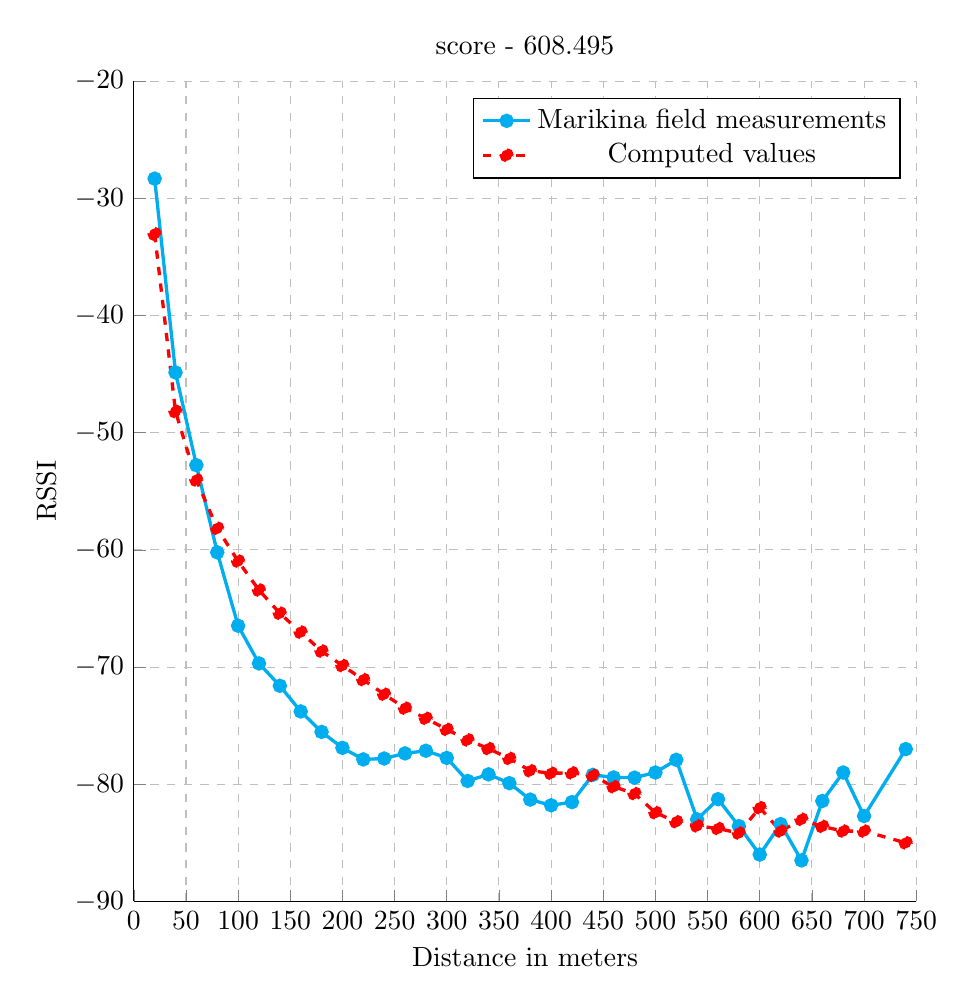
\begin{tikzpicture}%\label{plot:reachi-experiments:average-distance}
        \begin{axis}[
                title=score - 608.495,
                height=12cm, width=0.95\textwidth,
                ylabel={RSSI},
                xlabel={Distance in meters},
                axis lines*=left,
                xmin=0, xmax=750,
                enlargelimits=false,
                ymin=-90, ymax=-20,
                xtick={0, 50, 100, 150, 200, 250, 300, 350, 400, 450, 500, 550, 600, 650, 700, 750},
                ymajorgrids=true,
                xmajorgrids=true,
                grid style=dashed,
            ]

            \addplot[very thick, solid, cyan, mark=*] coordinates {(20, -28.32345013477089) (40, -44.85830258302583) (60, -52.77323717948718) (80, -60.21201657458563) (100, -66.47435897435898) (120, -69.68905472636816) (140, -71.5976496922216) (160, -73.7866473149492) (180, -75.53428571428572) (200, -76.89289392378991) (220, -77.88135593220339) (240, -77.8035019455253) (260, -77.36784140969164) (280, -77.14030612244898) (300, -77.75299760191847) (320, -79.71686746987952) (340, -79.15481171548117) (360, -79.90728476821192) (380, -81.30909090909091) (400, -81.79746835443038) (420, -81.52272727272727) (440, -79.2) (460, -79.42105263157895) (480, -79.4375) (500, -79.0) (520, -77.91666666666667) (540, -83.0) (560, -81.27272727272727) (580, -83.57142857142857) (600, -86.0) (620, -83.4) (640, -86.5) (660, -81.42857142857143) (680, -79.0) (700, -82.71428571428571) (740, -77.0)};
            \addlegendentry{Marikina field measurements};

            \addplot[very thick, dashed, red, mark=*] coordinates {(20,-33.04359925788497)(40,-48.19327731092437)(60,-54.03703703703704)(80,-58.16688567674113)(100,-60.96085858585859)(120,-63.43184421534937)(140,-65.41129831516353)(160,-67.02463054187191)(180,-68.64031007751937)(200,-69.87730061349693)(220,-71.07770961145194)(240,-72.32267441860465)(260,-73.50986842105263)(280,-74.37786259541984)(300,-75.32413793103449)(320,-76.22083333333333)(340,-76.95930232558139)(360,-77.8018018018018)(380,-78.84883720930233)(400,-79.06557377049181)(420,-79.03030303030303)(440,-79.25)(460,-80.21428571428571)(480,-80.8)(500,-82.42857142857143)(520,-83.2)(540,-83.55555555555556)(560,-83.77777777777777)(580,-84.16666666666667)(600,-82.0)(620,-84.0)(640,-83.0)(660,-83.6)(680,-84.0)(700,-84.0)(740,-85.0)};
            \addlegendentry{Computed values};
        \end{axis}
    \end{tikzpicture}
    \caption{Field measurements vs computed values}
    \label{plot:reachi-experiments:phili-log-vs-computed}
\end{figure}


\begin{figure}[H]
    \centering
    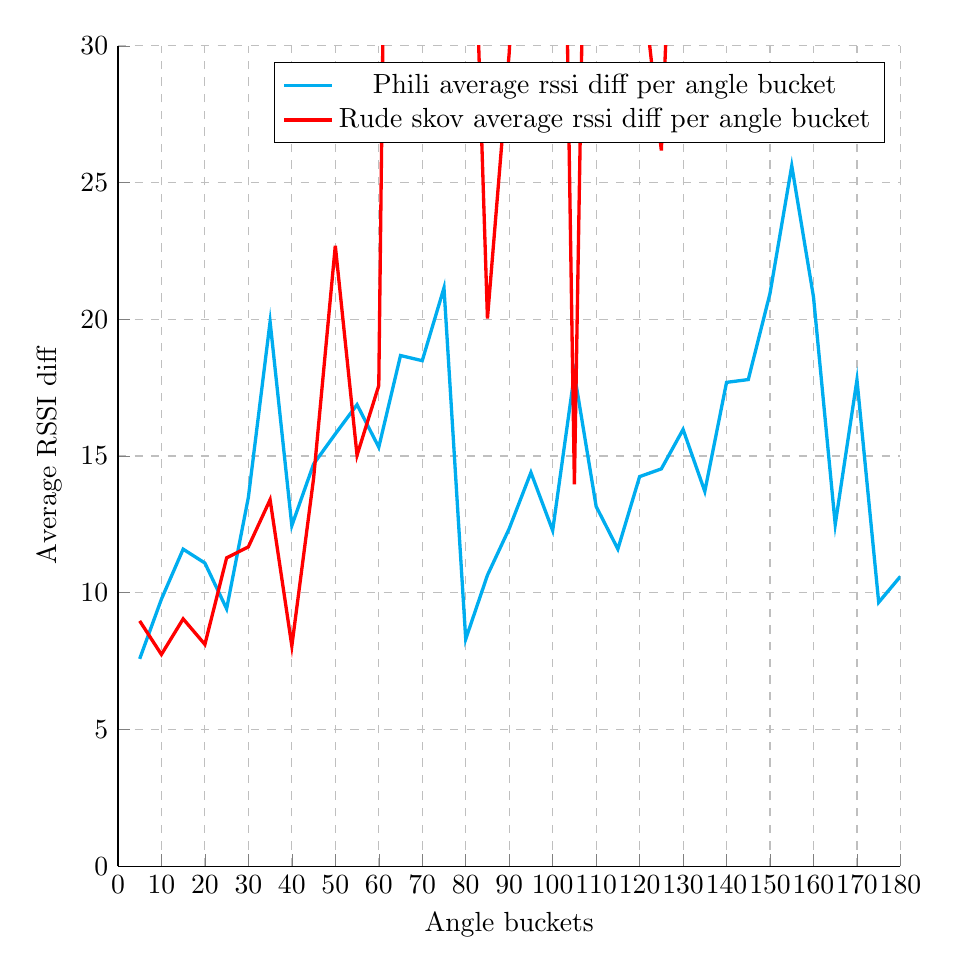
\begin{tikzpicture}%\label{plot:reachi-experiments:average-distance}
        \begin{axis}[
                height=12cm, width=0.95\textwidth,
                ylabel={Average RSSI diff},
                xlabel={Angle buckets},
                axis lines*=left,
                xmin=0, xmax=180,
                xtick={0, 10, 20, 30, 40, 50, 60, 70, 80, 90, 100, 110, 120, 130, 140, 150, 160,170,180},
                enlargelimits=false,
                ymin=0, ymax=30,
                ymajorgrids=true,
                xmajorgrids=true,
                grid style=dashed
            ]

            %\addplot[very thick, solid, cyan!50!black] coordinates {(5, 7.581215097994852) (10, 9.763581254686114) (15, 11.59234807189617) (20, 11.084399582147876) (25, 9.411670936293284) (30, 13.486232393853125) (35, 19.91110051641767) (40, 12.453590557884946) (45, 14.70313120243339) (50, 15.804939314638208) (55, 16.87697870999425) (60, 15.320902904198922) (65, 18.673392004683087) (70, 18.48508963612783) (75, 21.147550183881993) (80, 8.302184073487094) (85, 10.641508684206432) (90, 12.343183048128944) (95, 14.396643466792797) (100, 12.27504884861337) (105, 17.994872329043496) (110, 13.156645245862158) (115, 11.595967499573286) (120, 14.245146945189493) (125, 14.528392002600814) (130, 15.96981736460891) (135, 13.70427190114752) (140, 17.692009757218077) (145, 17.79486440192431) (150, 20.947579654378668) (155, 25.611175147469265) (160, 20.819124899373364) (165, 12.495568407794714) (170, 17.784042978338544) (175, 9.646875797269503) (180, 10.597197732034614)};
            \addplot[very thick, solid, cyan] coordinates {(5,7.581215097994852)(10,9.763581254686114)(15,11.59234807189617)(20,11.084399582147876)(25,9.411670936293284)(30,13.486232393853125)(35,19.91110051641767)(40,12.453590557884946)(45,14.70313120243339)(50,15.804939314638208)(55,16.87697870999425)(60,15.320902904198922)(65,18.673392004683087)(70,18.48508963612783)(75,21.147550183881993)(80,8.302184073487094)(85,10.641508684206432)(90,12.343183048128944)(95,14.396643466792797)(100,12.27504884861337)(105,17.994872329043496)(110,13.156645245862158)(115,11.595967499573286)(120,14.245146945189493)(125,14.528392002600814)(130,15.96981736460891)(135,13.70427190114752)(140,17.692009757218077)(145,17.79486440192431)(150,20.947579654378668)(155,25.611175147469265)(160,20.819124899373364)(165,12.495568407794714)(170,17.784042978338544)(175,9.646875797269503)(180,10.597197732034614)};
            \addlegendentry{Phili average rssi diff per angle bucket};


            %\addplot[very thick, solid, red!50!black] coordinates {(5, 8.968175725354994) (10, 7.741408675352775) (15, 9.042742837449076) (20, 8.108954051047618) (25, 11.273321343260399) (30, 11.67692967914715) (35, 13.401460743255232) (40, 8.053793318539391) (45, 14.17474549040368) (50, 22.68855220716477) (55, 15.026896145186285) (60, 17.5755161176863) (65, 85.01233086400362) (70, 59.69038212814202) (75, 62.41948703096457) (80, 44.72712810089782) (85, 20.029080610052482) (90, (29.737954905927445) (95, 43.39235466255519) (100, 64.720015835849) (105, 13.965589072181558) (110, 61.334883149884675) (115, 36.30455538419785) (120, 33.32223486902817) (125, 26.172354285886417) (130, 45.62355888699502) (135, 55.8474401182669) (140, 47.511612928722954) (145, 49.70429537245245) (150, 50.649080550831435) (155, 52.34402139529124) (160, 51.45218633523966) (165, 51.805898996936115) (170, 52.39131328924595) (175, 48.78102582759046) (180, 51.91529108595685)};
            \addplot[very thick, solid, red] coordinates {(5,8.968175725354994)(10,7.741408675352775)(15,9.042742837449076)(20,8.108954051047618)(25,11.273321343260399)(30,11.67692967914715)(35,13.401460743255232)(40,8.053793318539391)(45,14.17474549040368)(50,22.68855220716477)(55,15.026896145186285)(60,17.5755161176863)(65,85.01233086400362)(70,59.69038212814202)(75,62.41948703096457)(80,44.72712810089782)(85,20.029080610052482)(90,29.737954905927445)(95,43.39235466255519)(100,64.720015835849)(105,13.965589072181558)(110,61.334883149884675)(115,36.30455538419785)(120,33.32223486902817)(125,26.172354285886417)(130,45.62355888699502)(135,55.8474401182669)(140,47.511612928722954)(145,49.70429537245245)(150,50.649080550831435)(155,52.34402139529124)(160,51.45218633523966)(165,51.805898996936115)(170,52.39131328924595)(175,48.78102582759046)(180,51.91529108595685)};
            \addlegendentry{Rude skov average rssi diff per angle bucket};
        \end{axis}
    \end{tikzpicture}
    \caption{}
    \label{plot:reachi-experiments:avg-rssi-angle-phili-rude}
\end{figure}



\todo[inline]{show some plots, proving the problems}
\todo[inline]{talk about the visualiser + youtube link that shows the problems}
\todo[inline]{shortly mention CVPL and BOPL model that will be introduced in detail later}